\chapter{Orthogonalization}\label{chap:orthogonalisation}

\section{Introduction}\label{sec.approx-eig}

From Chapter~\ref{chap:jacobi_algorithm}, given a symmetric matrix $A\in\R\nn$, we can use the Jacobi algorithm to find an eigendecomposition $A = Q\varLambda Q\tp$. However, for large $n$, this procedure can still be time-consuming and is not generally as fast as the symmetric QR Algorithm~\ycite[2013, Section~8.5]{van2013mc}. However, the Jacobi algorithm can exploit the situation that $A$ is almost diagonal ($\off(A)$ is small). In 2000, Drma\u c and Veseli\'c proposed a way of speeding up this procedure using approximate eigenvectors as preconditioner~\ycite[2000, Section~1]{DRMAC2000-preconditioner}. They proposed the following
\begin{enumerate}
  \item Given a symmetric matrix $A\in\R\nn$ and its approximate orthogonal eigenvector matrix $Q_{\text{app}}$.
  \item Computing $A' = Q_{\text{app}}\tp A Q_{\text{app}}$.
  \item Diagonalizing $A'$.
\end{enumerate}
Suppose $Q_{\text{app}}$ is orthogonal in double precision and step 2 and 3 are carried out at double precision, then the eigenvalues we computed will have a small relative error and more efficient than the pure Jacobi method~\ycite[2000, Section~2]{DRMAC2000-preconditioner}. In this section, we will provide a way of constructing this approximate vector matrix:
\begin{enumerate}
  \item Compute the eigendecomposition at single precision such that 
  \begin{equation}\notag
    A = Q_\ell D_\ell Q_\ell\tp, \quad \norm{AQ_\ell - Q_\ell D_\ell} \lesssim nu_\ell \norm{A},\quad \norm{Q_\ell \tp Q_\ell - I} \lesssim nu_\ell,
  \end{equation}
  where $n$ is the dimension of the real symmetric matrix $A$ and $u_\ell$ is the unite roundoff at single precision. This can be achieved using \inline{eig} function in MATLAB via the following routine 
\begin{lstlisting}
[Q_low,D] = eig(single(A));
Q_low = double(Q_low);
\end{lstlisting}
  \item Orthogonalize the matrix $Q_\ell$ to $Q_d$ such that it is orthogonal at double precision,
  \begin{equation}\notag
    \norm{Q_d\tp Q_d - I} \lesssim nu_d.
  \end{equation}
\end{enumerate}

In this chapter, we will first review two methods to orthogonalize $Q_\ell$: the QR factorization and the polar decomposition. We aim to find the orthogonal (at double precision) matrix $Q_d$ that minimizes the norm $\norm{Q_d - U}$ where $U$ is the exact matrix of the eigenvectors of $A$. However, in practice, we have no access to the matrix $U$, therefore, we instead find the orthogonal matrix $Q_d$ that minimizes $\norm{Q_d - Q_\ell}$. This problem can be transformed to: Given $Q_\ell$, find the orthogonal matrix $Q_d$ such that it satisfies
\begin{equation}\notag
  \min{\norm{Q_\ell - Q_d}},\quad \text{under constraint: $\norm{Q_d\tp Q_d  = I}$.}
\end{equation}

Finally, the code in MATLAB will be presented and we will access them to decide which to use in practice.

\section{The Householder QR Factorization}\label{sec:Householder-QR}
The QR factorization of $A\in\R\nn$ is a factorization
\begin{equation}\notag
    A = QR
\end{equation}
where $Q\in\R\nn$ is orthogonal and $R\in\R\nn$ is upper triangular. Suppose we have a QR factorization at double precision of $Q_\ell$,
\begin{equation}\label{eq.2.2}
    Q_\ell = Q_d R,
\end{equation}
where $Q_d$ is orthogonal at double precision, and this is already our desired preconditioner. The QR factorization can be achieved using Householder transformations in Section~\ref{sec:Householder}. 

\subsection{Theory of Householder QR Factorization}\label{subsec.houseQR}

The idea can be illustrated using a small matrix $A\in\R^{4\times 4}$:
\begin{equation}\notag
    \begin{aligned}
    A &=
    \begin{bmatrix}
        \times & \times & \times & \times\\
        \times & \times & \times & \times\\
        \times & \times & \times & \times\\
        \times & \times & \times & \times
    \end{bmatrix}
    \stackrel{P_1 \in\R^{4\times 4}}{\longrightarrow}
    \begin{bmatrix}
        \times &\mid \times & \times & \times\\\hline
        0 &\mid \times & \times & \times\\
        0 & \mid\times & \times & \times\\
        0 & \mid\times & \times & \times\\
    \end{bmatrix}
    \stackrel{P_2 \in\R^{3\times 3}}{\longrightarrow}
    \begin{bmatrix}
        \times & \times & \times & \times\\
        0 & \times & \times & \times\\ \hline
        0 & 0 &\mid \times & \times\\
        0 & 0 & \mid \times & \times\\
    \end{bmatrix}\\
    & \stackrel{P_3 \in\R^{2\times 2}}{\longrightarrow}
    \begin{bmatrix}
        \times & \times & \times & \times\\
        0 & \times & \times & \times\\
        0 & 0 &\times & \times\\
        0 & 0 & 0 & \times\\
    \end{bmatrix} = R,
    \end{aligned}
\end{equation}
where $P_k$, $k = 1,2,3$, are the Householder transformations. Notice that $P_2\in\R^{3\times 3}$ only applies to the bottom right corner of the matrix, and this can be done by embedding $P_2$ inside a larger $4\times 4$ matrix via
\begin{equation}\notag
    \wt P_2 =
    \begin{bmatrix}
        1 & 0 \\
        0 & P_2
    \end{bmatrix}
\end{equation}

Hence from the example above, we can generalize the Householder QR factorization for $A\in\R\nn$. It will produce a sequence of matrices $\{A_k\}_{k=1}^{n}$ where $A_1$ is the input $A$ and $A_n$ is the upper triangular matrix $R$. Notice, there are $k-1$ stages where the $k$th stage transform $A_k$ to $A_{k+1}$.

At the $k$th stage of the Householder QR factorization, we can carefully partition the matrix $A_k$ into the following form

\begin{equation}\notag
    A_{k} =
    \begin{bmatrix}
        R_{k-1} & w_k & C_k \\
        0 & x_k & B_k
    \end{bmatrix},
    \quad R_{k-1}\in\R^{(k-1)\times (k-1)}, x_k\in\R^{n-k+1},
\end{equation}
where $R_{k-1}$ is upper triangular (achieved at the ($k-1$)th stage) and $x_k$ is the vector that we should focused on the $k$th stage. Choose a Householder transformation $P_k$ such that $P_kx_k = \sign{x_{k,1}}\norm{x_k}e_1$, where $e_1$ is the first column of $I_{n-k+1}$ and $x_{k,1}$ is the first entry of the vector $x_k$. We then embed matrix $P_k$ into a larger matrix $\wt P_k\in\R\nn$ via
\begin{equation}\label{eq.qrQ}
    \wt P_k =
    \begin{bmatrix}
        I_{k-1} & 0 \\
        0 & P_k
    \end{bmatrix},\quad P_k \in \R^{(n-k+1)\times(n-k+1)}.
\end{equation}
Then let $A_{k+1} = \wt P_k A_k$, we have 
\begin{equation}\label{eq.qrstep}
    A_{k+1} = 
    \begin{bmatrix}
        R_{k-1} & w_k & C_k \\
        0 & P_k x_k & P_k B_k
    \end{bmatrix}
     = 
     \begin{bmatrix}
        R_{k-1} & w_k & C_k \\
        0 & \sign{x_{k,1}}\norm{x_k}e_1 & P_k B_k
     \end{bmatrix},
\end{equation}
which is closer to the upper triangular form. After $n-1$ steps, the matrix $A_{n}$ will be upper triangular and we denote as $R$ and we obtain the QR factorization of $A$
\begin{equation}\notag
    A_{n-1} = R = \wt P_{n-1}\wt P_{n-2} \cdots \wt P_1 A =: Q\tp A.
\end{equation}
Since $\wt P_k$ are composed of $P_k$, Householder matrices, and the identity matrix. Hence it is obvious that $\wt P_k$ are also symmetric and orthogonal. Then we can construct $Q$ via $\wt P_1 \cdots\wt P_{n-1}$. This procedure can be summarized in the Algorithm~\ref{alg:householderQR}.

\begin{algorithm}[ht]
\caption{Given $A\in\R\nn$, this algorithm computes an orthogonal matrix $Q$ and an upper triangular matrix $R$ such that $A = QR$.} \label{alg:householderQR}
\begin{algorithmic}[1]
    \State{$Q = I_n$}
    \For {$k=1:n-1$}
        \State{$[v,\beta] = \mathtt{house}(A(k:n,k))$} \Comment{From Algorithm~\ref{alg.house}}
        \State{$A(k:n,k:n) = (I_{n-k+1}-\beta vv\tp )A(k:n,k:n)$}
        \State{$Q(1:n,k:n) = Q(1:n,k:n)(I_{n-k+1}-\beta vv\tp)$}
    \EndFor
\end{algorithmic}
\end{algorithm}

Line $4$ is directly adapted from~\eqref{eq.qrstep}. Line $5$ can be viewed by partitioning the orthogonal matrix $Q_k$ into four parts and multiplying the matrix $\wt P_k$ structured as~\eqref{eq.qrQ},
\begin{equation}\label{eq:update-Q}
    Q_{k+1} = Q_k\wt P_k = 
    \begin{bmatrix}
        Q_1 & Q_2 \\
        Q_3 & Q_4
    \end{bmatrix}
    \begin{bmatrix}
        I_{k-1} & 0 \\
        0 & P_k
    \end{bmatrix} = 
    \begin{bmatrix}
        Q_1 & Q_2 P_k \\
        Q_3 & Q_4 P_k
    \end{bmatrix}.
\end{equation}
Hence, at each step of the algorithm, we only update the final $n-k+1$ columns of the matrix $Q_k$. Also, focused on the line 4, if we construct $P$ and do a matrix-matrix multiplication between $D_k,P_k\in\R^{(n-k+1)\times (n-k+1)}$ where $D_k = [x_k,B_k]$, then the cost will be about $2(n-k+1)^3$. If we utilize the components we computed from Algorithm~\ref{alg.house}, the Householder vector $v$ and the coefficient $\beta$, we can reduce the computational cost by doing the matrix-vector products instead. We can rewrite $P_k D_k$ using $v$ and $\beta$
\begin{equation}\notag
    P_k D_k = (I - \beta vv\tp) D_k = D_k - \beta v v\tp D_k = D_k - (\beta v)\cdot(v\tp D_k).
\end{equation}
By this procedure, we transform a matrix-matrix multiplication to
\begin{enumerate}
    \item Vector-matrix multiplication: $v\tp D_k$ requires $2(n-k+1)^2$ flops.
    \item Scalar-vector inner product: $\beta v$ requires $O(n-k+1)$ flops.
    \item Vector-vector outer product: $(\beta v)\cdot (v\tp D_k)$ requires $(n-k+1)^2$ flops.
    \item Matrix-matrix subtraction: $D_k - (\beta v)\cdot(v\tp D_k)$ requires $O(n-k+1)^2$ flops.
\end{enumerate}
Therefore, the overall cost will be $4(n-k+1)^2$ flops. Compare with the matrix-matrix multiplication which requires $O((n-k+1)^3)$ flops, this approach is much more efficient.

\subsection{Implementation and Testing}\label{sec.qrtesting}
Based on these analyses in Section~\ref{subsec.houseQR}, we can implement it into \mat.

\begin{lstlisting}
function [Q,A] = myqr(A)
[m,n] = size(A); Q = eye(n);
if m ~= n, error('Input should be a square matrix.'), end
for k = 1:n-1
    [v,b] = house(A(k:n,k)); % compute the components of P
    A(k:n,k:n) = A(k:n,k:n) - (b*v)*(v'*A(k:n,k:n)); % update A
    Q(:,k:n) = Q(:,k:n) - (Q(:,k:n)*v)*(b*v'); % update Q
end
\end{lstlisting}

Recall from the last section, we discussed that at the $k$th step, updating $A$ requires about $4(n-k+1)^2$ flops. Similarly, we can update $Q$ based on~\eqref{eq:update-Q} which only involves $(n-k+1)$ columns of $Q$. Therefore, line 7 requires $4(n-k+1)n$ flops at the $k$th step. We can then compute the theoretical overall cost,
\begin{equation}\notag
    \text{Cost} = \sum_{k = 1}^{n-1} 4(n-k+1)^2 + 4(n-k+1)n = O(10n^3/3).
\end{equation}


To test our code, we are focused on two quantities, $\norm{Q\tp Q - I}$ and $\norm{QR - A}$. The former evaluates whether our computed $Q$ is orthogonal at double precision and the latter evaluates whether we have a QR factorization. In theory, we should have 
\begin{equation}\notag
    \norm{Q\tp Q - I} \lesssim nu_d, \quad \norm{QR - A}/\norm{A} \lesssim nu_d.
\end{equation}
We can use the following MATLAB routine, notice that we add the accuracy of the MATLAB built-in function \inline{qr} as a reference.
\begin{lstlisting}
clc; clear; format short e; 
n = 1e2; ud = 2^(-53); A = randn(n); 
[Q,R] = myqr(A); [Q1,R1] = qr(A); % qr factorization
orthg = norm(Q'*Q - eye(n)); % check orthogonality
qralg = norm(Q*R - A)/norm(A); % check if we have a qr factorization
fprintf('Orthogonal? %d \nMy QR accuracy is %d\n',orthg, qralg);
fprintf('MATLAB qr function accuracy is %d \n', norm(Q1*R1 - A)/norm(A));
fprintf('n*(machine precision) = %d\n', ud*n);
\end{lstlisting}
And we have the output:
\begin{lstlisting}
Orthogonal? 3.567685e-15 
My QR accuracy is 1.493857e-15
MATLAB qr function accuracy is 1.026458e-15 
n*(machine precision) = 1.110223e-14
\end{lstlisting}

The first and second outputs are all smaller than $nu_d \approx 10^{-13}$ therefore our code works well. In addition, the second and the third outputs are the accuracy of functions \inline{myqr} and \inline{qr} and we can see these are about the same, therefore our code achieves similar accuracy as the MATLAB built-in function.

Moreover, I am interested in how $\norm{Q\tp Q - I_n}$ behaved as $n$ increases. From Figure~\ref{fig:orthog}, we can see $\norm{Q\tp Q - I_n}$ does not increase too much when $n$ increases and is well bounded by the reference line $nu_d$.

\begin{figure}[ht]
    \centering 
    \includegraphics[width=0.5\textwidth]{figs/myqr-numerical-test.pdf}
    \caption[Behavior of $\norm{Q\tp Q - I_n}$ with $n$ increases and $\kappa(A)$ fixes using the Householder QR factorization.]{Behavior of $\norm{Q\tp Q - I_n}$ with $n$ increases from $100$ to $3000$ with step size $100$ and $\kappa(A) = 100$ using my own QR code \inline{myqr}. The red line shows the computed results and the black line shows the reference line $nu_d$. The code to regenerate this graph can be found in Appendix~\ref{app:fig:orthog}.}
    \label{fig:orthog}
\end{figure}

By now, we have a way to orthogonalize a matrix. However, this approach does not utilize the property that our input matrix $Q_\ell$ is an almost orthogonal matrix. Namely, applying \inline{myqr} to $Q_\ell$ has no difference from applying \inline{myqr} to a general matrix. In the next section, we will introduce a way to orthogonalize a matrix which exploits the fact that the input is almost orthogonal.


\section{The Polar Decomposition}\label{sec:polar-decomposition}

In complex analysis, it is known that for any $\alpha\in\C$, we can write $\alpha$ in polar form, namely $\alpha = r\eu^{\im \theta}$. The polar decomposition is its matrix analogue. The polar decomposition can be derived from the singular value decomposition discussed in Section~\ref{sec:svd}. Conventionally, we will present our analysis in complex but this can be restricted to real. All the norm $\gnorm{\cdot}$ discussed in this section will be the orthogonally invariant norm.


\begin{theorem}
    [Polar decomposition]
    \label{thm.polar-decompo}
    If $A\in\C\nn$, then there exists a unitary matrix $U\in\C\nn$ and a unique Hermitian positive semidefinite matrix $H\in\C\nn$ such that $A = UH$. We call $U$ the unitary factor.
\end{theorem}

\begin{proof}
    By Theorem~\ref{thm.svd}, suppose $A\in\C\nn$ and $\rank(A) = r$, then the SVD of $A$ can be written as 
    \begin{equation}\label{eq.polar-decomp-factors}
        A = P\varSigma_r V\ctp = 
        \underbrace{PV\ctp}_{U} 
        \underbrace{
        V \Sigma_r
        V\ctp}_{H}
        \equiv UH,
    \end{equation}
    where $\Sigma_r = \diag(\sigma_1,\dots,\sigma_r,0,\dots,0)\in\R\nn$.
    Unitarity of $U$ can be easily proved by its definition 
    \begin{equation}\notag
        UU\ctp = PV\ctp VP\ctp = I_n,\quad U\ctp U = VP\ctp P V\ctp = I_n.
    \end{equation}
    $H$ is a positive semidefinite due to its eigenvalues are the singular values of $A$ which are all non-negative. By forming $A\ctp A$, we have $A\ctp A = H\ctp U\ctp U H = H\ctp H = H^2$, therefore $H$ can be uniquely determined by $(A\ctp A)^{1/2}$~\ycite[2008, Theorem~1.29]{higham08fm}.
\end{proof}

Notice that, if $A$ is full rank, then $H$ is clearly non-singular by construction, therefore $U$ can be uniquely determined by $U = AH\inv$. Similar to the QR factorization, we have a decomposition of $A$ where one of the factors is unitary, and we expect that we can use this unitary factor as the preconditioner. The next section gives a special property which shows the unitary factor $U$ of the polar decomposition of $A$ is the one that minimizes the distance $\gnorm{A-U}$.

\subsection{Best Approximation Property}

The unitary factor $U$ of the polar decomposition of $A = UH$ satisfies the best approximation property.

\begin{theorem}[{\ycite[1955, Theorem~1]{Fan-Hoffman},\ycite[2008, Theorem~8.4]{higham08fm}}]
    \label{thm.best_approx}
    Let $A\in\C\nn$ and $A= UH$ is its polar decomposition. Then 
    \begin{equation}\notag
        \gnorm{A-U} = \min\left\{\gnorm{A-Q}\mid Q\ctp Q = I_n\right\}
    \end{equation}
    holds for every unitarily invariant norm.
\end{theorem}

To prove Theorem~\ref{thm.best_approx}, we need the following two results:

\begin{lemma}[{\ycite[1960, Lemma~4]{Lemma4-Theorem5-Mirsky}}]
    \label{lemma.3.2}
    Let $X, Y$ be Hermitian matrices, and denote by 
    \begin{equation}\notag
        \xi_1\geq \cdots \geq \xi_n,\quad 
        \eta_1 \geq \cdots \geq \eta_n,\quad 
        \zeta_1\geq \cdots \geq \zeta_n
    \end{equation}
    be the eigenvalues of $X, Y$ and $X-Y$ respectively. Then if we denote by $(\xi-\eta)_1,\dots,(\xi-\eta)_n$ the numbers $\xi_1 -\eta_1,\dots,\xi_n-\eta_n$ arranged in non-ascending order of magnitude, then we have
    \begin{equation}\notag
        \sum_{i=1}^k (\xi-\eta)_i \leq \sum_{i=1}^k(\zeta_i), \quad 1\leq k\leq n.
    \end{equation}
\end{lemma}

\begin{proof}
    See \ycite[1955, Theorem~2]{Lemma4proof}
\end{proof}

\begin{theorem}[{\ycite[1960, Theorem~5]{Lemma4-Theorem5-Mirsky}, \ycite[2008, Theorem~B.3]{higham08fm}}]
    \label{thm.3.3}
    Let $\rho_1\geq \cdots\geq\rho_n$ and $\sigma_1\geq \cdots\geq \sigma_n$ be the singular values of the complex matrices $A$ and $B$ respectively. Then 
    \begin{equation}\notag
        \gnorm{A-B}\geq \gnorm{\Sigma_A - \Sigma_B},
    \end{equation}
    where $\Sigma_A$ and $\Sigma_B$ are diagonal matrices with entries the singular values of $A$ and $B$ arranged in non-ascending order respectively.
\end{theorem}

\begin{proof}
    We have the fact by H. Wielandt mentioned in~\ycite[1955, p.~113]{Fan-Hoffman}: For any matrix $M$ of order $n\times n$, the Hermitian matrix 
    \begin{equation}\notag
        \wt M = 
        \begin{bmatrix}
            0 & M\\
            M\ctp & 0
        \end{bmatrix}
    \end{equation}
    of order $2n\times 2n$. The eigenvalues of $\wt M$ are precisely the singular values of $M$ and their negatives. We denote $\tau_1 \geq \cdots \geq \tau_n$ the singular values of $A-B$ and we have 
    \begin{equation}\notag
        \begin{bmatrix}
            0 & A \\
            A\ctp & 0
        \end{bmatrix}
        -
        \begin{bmatrix}
            0 & B\\
            B\ctp & 0
        \end{bmatrix}
        =
        \begin{bmatrix}
            0 & A-B\\
            A\ctp - B\ctp & 0
        \end{bmatrix}
    \end{equation}
    and the eigenvalues of these three Hermitian matrices are 
    \begin{equation}\notag
        \begin{aligned}
            \rho_1\geq\cdots\geq\rho_n &\geq -\rho_n\geq \cdots\geq -\rho_1, \\
            \sigma_1\geq\cdots\geq\sigma_n&\geq -\sigma_n\geq \cdots\geq -\sigma_1, \\
            \tau_1\geq\cdots\geq\tau_n&\geq -\tau_n\geq \cdots\geq -\tau_1.
        \end{aligned}
    \end{equation}
    By Lemma~\ref{lemma.3.2}, if we denote $(\rho-\sigma)_1,\dots,(\rho-\sigma)_n$ the numbers $\rho_1 -\sigma_1,\dots,\rho_n-\sigma_n$ arranged in non-ascending order of magnitude, then we have 
    \begin{equation}\notag
        \sum_{i=1}^k \tau_i \geq \sum_{i=1}^k (\rho - \sigma)_i,\quad 1\leq k \leq n.
    \end{equation}
    Here we focus on the proof for $2$-norm, to see the proof considering all the orthogonally invariant norms, refer to~\ycite[1960, Theorem~1]{Lemma4-Theorem5-Mirsky}. By Corollary~\ref{col.2norm}
    \begin{equation}\notag
        \begin{aligned}
            \norm{A-B} &  = \norm{\diag\{\tau_1,\dots,\tau_n\}} = \tau_1 \\
            & \geq (\rho - \sigma)_1 = \max_k{\abs{\rho_k - \sigma_k}}\\
            & = \norm{\diag\{{\rho_1-\sigma_1},\dots,{\rho_n-\sigma_n}\}} \\
            & = \norm{\Sigma_A - \Sigma_B} \qedhere
        \end{aligned} 
    \end{equation}
\end{proof}

\begin{proof}
    [Proof of Theorem~\ref{thm.best_approx}]
    For any unitary matrix $Q$, it has singular values all equal to $1$. Hence by Theorem~\ref{thm.3.3}, if $A$ has the singular value decomposition $A=P\Sigma_A V\ctp$, then $$\gnorm{A-Q}\geq\gnorm{\Sigma_A - I_n}.$$
    Remain to prove that $\gnorm{A-U} = \gnorm{\Sigma_A - I_n}$. From Theorem~\ref{thm.polar-decompo}, the Hermitian part $H$ can be written as $V\Sigma_A V\ctp$, hence 
    \begin{equation}\notag
        \gnorm{A-U} = \gnorm{U(H-I_n)} = \gnorm{H-I_n} = \gnorm{V \Sigma_A V\ctp - I_n} = \gnorm{\Sigma_A - I_n},
    \end{equation}
    which completes the proof.
\end{proof}

This property indicates that the unitary factor of the input $Q_\ell$ will be the desired orthogonal matrix and then we can use it as the preconditioner. The rest of this section will focus on how to compute this factor.

\subsection{SVD approach}\label{sec:svdapproach}

The most obvious approach will be the singular value decomposition approach.

For $A\in\C\nn$, by Theorem~\ref{thm.polar-decompo}, we can use the singular value decomposition to compute the polar decomposition using the following procedure:
\begin{enumerate}
    \item Compute the singular value decomposition of $A\in\C\nn$ where $A = P\Sigma V\ctp$.
    \item Form $U$ via~\eqref{eq.polar-decomp-factors}, $U = P V\ctp$.
\end{enumerate}
The computational cost of computing the singular value decomposition is approximately $21n^3$ flops \ycite[2013, Figure~8.6.1]{van2013mc} with $O(n^3)$ flops to form $U$. This is good generally, but it does not utilize the property that, in our scenario, $A$ is almost orthogonal ($\norm{A\ctp A - I_n}$ is small). The next two sections will discuss a more sophisticated way of computing the unitary factor.

\subsection{Newton's Method Approach}

Consider the Newton iteration~\ycite[2008, Section~8.3]{higham08fm}
\begin{equation}\label{eq.iter}
    \begin{aligned}
        X_0 &= A\in\C\nn, \text{nonsingular}\\
        X_{k+1} &= \frac{1}{2}(X_k + X_k^{-*}),\quad k = 0,1,\dots,
    \end{aligned}
\end{equation}
where $(X_k^{-*})$ denotes the conjugate transpose of the inverse of $X$. The following theorem shows the iteration~\eqref{eq.iter} converges to the unitary factor of $A$.
\begin{theorem}
    [Newton iteration for the unitary polar factor]
    \label{thm.newton-iteration}
    Suppose $A\in\C\nn$ is nonsingular, then the iteration~\eqref{eq.iter} produces a sequence $\{X_k\}_k$ such that 
    \begin{equation}\notag
        \lim_{k\to\infty} X_k = U,
    \end{equation}
    where $U$ is the unitary factor of the polar decomposition of $A$.
\end{theorem}

\begin{proof}
    See \ycite[1986, Section~3.2]{NJH86Polar}.

    Let the singular value decomposition of $A$ be $P \Sigma Q\ctp$, where $P$ and $Q$ are unitary. Then by Theorem~\ref{thm.polar-decompo}, we have $A = UH$ where $U = PQ\ctp$ and $H = Q\Sigma Q\ctp$. The trick of the proof is to define a new sequence ${D_k}$ where 
    \begin{equation}\label{eq.XtoD}
        D_k = P\ctp X_k Q.
    \end{equation}
    From iteration~\eqref{eq.iter}, we have 
    \begin{equation}\notag
        \begin{aligned}
            D_0 &= P\ctp X_0 Q = P\ctp AQ = \Sigma,\\
            D_{k+1} &= P\ctp X_{k+1} Q = P\ctp \frac 12 (X_k + X_k^{-*})Q \\
            & = \frac 12 (P\ctp X_k Q + P\ctp X_k^{-*}Q).
        \end{aligned}
    \end{equation}

    Notice that $P\ctp X_k Q = D_k$ and $P\ctp X_k^{-*}Q = (P\ctp X_k Q)^{-*}$, hence the iteration becomes 
    \begin{equation}\label{eq.iterD}
        \begin{aligned}
            D_0 = \Sigma, \quad D_{k+1} = \frac 1 2 (D_k + D_k^{-*}).
        \end{aligned}
    \end{equation}
    Since $D_0$ is diagonal with positive diagonal entries (since $A$ is full rank), hence the iteration~\eqref{eq.iterD} is well-defined and will produce a sequence of diagonal matrices $\{D_k\}$ and we can write $D_k = \diag(d_i^{(k)})$, where $d_i^{(k)} > 0$. Using this notation, we can rewrite the iteration~\eqref{eq.iterD} elementwise:
    \begin{equation}\notag
        d_i^{(0)} = \sigma_i,\quad d_i^{(k+1)} = \frac 12 \left(d_i^{(k)} + \frac{1}{d_i^{(k)}}\right)
    \end{equation}
    where $i = 1,\dots,n$. By an argument discussed in \ycite[1964, p.~84]{Henrici1964ElementofNA}, we can write 
    \begin{equation}\label{thm.conv-proof1}
        \begin{aligned}
        d_i^{(k+1)} - 1 = \frac{1}{2d_i^{(k)}}\left({d_i^{(k)}}^2 -2d_i^{(k)} + 1 \right) = \frac{1}{2d_i^{(k)}} \left(d_i^{(k)}-1\right)^2
        \end{aligned}
    \end{equation}
    This implies that the diagonal entries of $D_k$ converge to $1$ quadratically as $k\to\infty$. Since the argument holds for any $i  = 1,\dots,n$, we conclude that $\lim_{k\to\infty} D_k = I_n$ and use the definition of $D_k$ we have 
    \begin{equation}\notag
        \lim_{k\to\infty} X_k = PD_k Q\ctp = PQ\ctp = U,
    \end{equation}
    as $k\to\infty$, where $U$ is the unitary factor of the polar decomposition of $A$.
\end{proof}

The Newton iteration for the unitary factor of a square matrix $A$ can also be derived by applying the Newton's method to the equation $X\ctp X = I_n$. Consider a function $F(X) = X\ctp X - I_n$, then $X$ is unitary if $X$ is a zero of the function $F(X)$. 

Suppose $Y$ is an approximate solution to the equation $F(\wt X) = 0$, we can write $\wt X = Y + E$ and substitute $\wt X$ into the equation $F(\wt X) = 0$
\begin{equation}\notag
    (Y+E)\ctp (Y+E) - I_n = Y\ctp Y + Y\ctp E + E\ctp Y + E\ctp E - I_n = 0.
\end{equation}
Dropping the second order term, we get Newton iteration $Y\ctp Y + Y\ctp E + E\ctp Y - I_n = 0$ and this is the Sylvester equation for $E$~\ycite[2008, Problem~8.18]{higham08fm}. We aim to solve $E$ and update $Y$ by $Y + E$, which gives the Newton iteration at the $k$th step:
\begin{equation}\label{eq.it1}
    \begin{cases}
        X_k \ctp X_{k} + X_{k}\ctp E_k + E_k\ctp X_k - I_n = 0,\\
        X_{k+1} = X_{k} + E_k.
    \end{cases}
\end{equation}
Assume that $X_k\ctp E_k$ is Hermitian, namely $X_k\ctp E_k = E_k\ctp X_k$, then we can further simplify the iteration by rewritten~\eqref{eq.it1} as $X_k\ctp E_k = (I_n - X_k\ctp X_k)/2$ and the expression we got for $X_k\ctp E_k$ is indeed Hermitian, hence our assumption is valid. Therefore, we have a explicit expression for $E_k$, $E_k = (X_k^{-*} - X_k)/2$, and the iteration~\eqref{eq.it1} becomes 
\begin{equation}\notag
    X_{k+1} = X_{k} + \frac 12 (X_k^{-*}-X_k) = \frac 12(X_k^{-*} + X_k)
\end{equation}
choosing $X_0 = A$, we have our desired Newton iteration~\eqref{eq.iter}.

\subsubsection{Convergence of Newton Iteration}

The convergence of the iteration~\eqref{eq.iter} can be seen from the proof of Theorem~\ref{thm.newton-iteration}.

\begin{theorem}
    [Convergence of the iteration~\eqref{eq.iter}, {\ycite[2008, Theorem~8.12]{higham08fm}}] \label{thm.conv.new}
    Let $A\in\C\nn$ be non-singular. Then the Newton iterates $X_k$ in~\eqref{eq.iter} converges quadratically to the unitary polar factor $U$ of $A$ with 
    \begin{equation}\notag
        \gnorm{X_{k+1} - U} \leq \frac 12 \gnorm{X_k\inv}\gnorm{X_k - U}^2,
    \end{equation}
    where $\gnorm{\cdot}$ is any unitarily invariant norm.
\end{theorem}

\begin{proof}
    Given $A\in\C\nn$, the singular value decomposition of $A$ is $P\Sigma Q\ctp$ and the unitary factor is $U = PQ\ctp$. From~\eqref{thm.conv-proof1}, we have 
    \begin{equation}\notag
        d_i^{(k+1)} - 1 = \frac{1}{2d_i^{(k)}}\left(d_i^{(k)}-1\right)^2.
    \end{equation}
    This is true for all $1\leq i\leq n$, therefore we can rewrite this in matrix form
    \begin{equation}\label{eq.3.28}
        \begin{bmatrix}
            d_1\iter{k+1}-1 & & \\
            & \ddots & \\
            & & d_n\iter{k+1}-1
        \end{bmatrix} = 
        \frac{1}{2}
        \begin{bmatrix}
            1/d_1\iter{k} & & \\
            & \ddots & \\
            & & 1/d_n\iter{k}
        \end{bmatrix}
        \begin{bmatrix}
            d_1\iter{k}-1 & & \\
            & \ddots & \\
            & & d_n\iter{k}-1
        \end{bmatrix}^2
    \end{equation}

    Recall $D_k = \diag(d_i\iter{k})$, then~\eqref{eq.3.28} is same as $D_{k+1}-I = D_k\inv (D_k - I)^2/2$. Therefore we can conclude that $D_{k}$ converges to the identity $I$ quadratically and therefore $X_{k}$ converges to the unitary factor $U$ quadratically.

    From $D_{k+1}-I = D_k\inv (D_k - I)^2/2$, by taking the norm on both sides we have 
    \begin{equation}\label{eq.Dineq}
        \begin{aligned}
            \gnorm{D_{k+1}-I} &= \frac 12 \gnorm{D_k\inv (D_k - I)^2} \leq \frac 12 \gnorm{D_k\inv} \gnorm{D_k - I}^2
        \end{aligned}
    \end{equation}
    The final inequality comes from the fact that every unitarily invariant norm is subordinate~\ycite[1997, Proposition~IV~2.4]{1997-matrix-analysis}. Also, the unitary invariance implies the following three equalities,
    \begin{itemize}
        \item $\gnorm{D_{k+1}- I} = \gnorm{PD_{k+1} Q\ctp - PQ\ctp} = \gnorm{X_{k+1} - U}$. 
        \item $\gnorm{D_k\inv} = \gnorm{QD_k\inv P\ctp} =\gnorm{X_k\inv}$.
        \item Using the same argument as 1, we have $\gnorm{D_k - I} = \gnorm{X_k - U}$.
    \end{itemize}
    As a result, \eqref{eq.Dineq} can be rewritten as 
    \begin{equation}\notag
        \gnorm{X_{k+1} - U} \leq \frac 12 \gnorm{X_k\inv}\gnorm{X_k - U}^2.
    \end{equation}
\end{proof}

We can test the iteration~\eqref{eq.iter} by the following code 
\begin{lstlisting}
A = my_testmatrices(10,100); X = A;
for i = 1:10
    Y = inv(X);
    X = (Y' + X)/2;
end
[P,~,V] = svd(A); U = P*V'; 
disp(norm(X-U));
\end{lstlisting}
With only $10$ iterations, the distance between our computed polar factor and the theoretical polar factor (formed by singular value decomposition) is as small as the unit roundoff. However, the disadvantage of this iteration is that it requires the explicit form of the inverse of a matrix at each step, therefore we can introduce another method using one step of the Schulz iteration~\ycite[1965]{Adi1965-MatrixInverse} which will remove the requirement of the matrix inverse.

\subsection{Newton--Schulz Iteration Approach}

Given $A\in\C\nn$, an iterative method for computing the inverse $A\inv$, proposed by Schulz \ycite[1933, p.~58]{Schulz1933}, is defined by 
\begin{equation}
    \label{eq.schuiter}
    X_{k+1} = X_{k}(2I - AX_k), \quad k = 0,1,2,\dots,
\end{equation}
where $X_0$ is an approximation to $A\inv$. Based on the \eqref{eq.iter}, we can use a one-step Schulz iteration to approximate the inverse of $X_k\ctp$ which can be written as $Y_1 = Y_0(2I - X_k\ctp Y_0)$, where $Y_0$ is an approximation to $X_k^{-*}$. In our situation, the input $X_0$ is an almost unitary matrix ($\norm{X_0\ctp X_0 - I}$ is small) and the output is $U$ which is unitary. Hence the sequence generated by the Newton iteration, $\{X_k\}$, should always be almost unitary, therefore $X_k$ should be a good approximate to $(X_k\ctp)\inv$. The idea of Newton--Schulz iteration can be formulated by the Algorithm~\ref{alg:ns1}.
\begin{algorithm}[ht]
\caption{Given $A\in\C\nn$ such that $\norm{A\ctp A - I} \approx u_\ell$, the algorithm computes the unitary factor $U$ of $A$ defined by Theorem~\ref{thm.polar-decompo}.}
\label{alg:ns1}
\begin{algorithmic}[1]
    \State{$X_0 = A$}
    \For{$k = 0,1,2,\dots$}
        \State{$X_k^{-*} = X_k(2I - X_k\ctp X_k)$} \Comment{One-step Schulz iteration}
        \State{$X_{k+1} = \frac{1}{2}\left(X_k^{-*} + X_k\right)$} \Comment{Newton iteration}
    \EndFor
\end{algorithmic}
\end{algorithm}

Notice that, the one-step Schulz iteration can be embedded into the Newton iteration by substituting the $X_k^{-*}$ from line $3$ into line $4$ and we have 
\begin{equation}\label{eq.itNS}
    X_{k+1} = \frac{1}{2}\left(X_k(2I - X_k\ctp X_k) + X_k\right) = \frac 12 X_k\left(3I - X_k\ctp X_k\right), \quad X_0 = A,
\end{equation}
and this is known as the Newton--Schulz iteration~\ycite[2008, Section~8.3]{higham08fm}.

\subsubsection{Convergence of Newton--Schulz Iteration}

We would like to know, the iteration~\eqref{eq.itNS} converges to $1$ under which condition. Using the similar approach as proof of Theorem~\ref{thm.newton-iteration}, by writing $D_k = P\ctp X_k Q$ where $P$ and $Q$ are the unitary parts of the singular value decomposition of $A = P\Sigma Q\ctp$, we can consider the iteration~\eqref{eq.itNS} as the scalar form:
\begin{equation}\label{NSscalar}
    d_i\iter{k+1} = \frac 12 d_i\iter{k}\left(3-{d_i\iter{k}}^2\right),\quad d_i\iter{0} = \sigma_i,\quad \text{for $k=0,1,\dots,$}
\end{equation}
where $\sigma_i$ is the $i$th singular value of $A$. To see the convergence of~\eqref{eq.itNS}, we first find the interval of convergence of~\eqref{NSscalar}.

\begin{lemma}\label{lemma.scalarNS}
    If $\sigma_i\in (0,\sqrt{3})$, then the iteration~\eqref{NSscalar} converges quadratically to $1$.
\end{lemma}

\begin{proof}
    If $\sigma_i = 1$, then the iteration converges immediately. To simplify the notation, we rewrite the iteration~\eqref{NSscalar} as 
    \begin{equation}\label{eq.3.34}
        d_{k+1} = f(d_k) = \frac 12 d_k(3-d_k^2),\quad k = 0,1,\dots.
    \end{equation}
    \quad \textit{Case 1:} If $d_k\in (0,1)$, then $(3-d_k^2)/2 > 1$ which gives $d_k(3-d_k^2)/2 > d_k$. Differentiate $f(d_k)$ once we have $f'(d_k) = -d_k^2 +(3-d_k^2)/2$ and this will always be positive for $d_k\in(0,1)$. Therefore, if we start with $d_k\in (0,1)$, then $d_k < f(d_k) = d_{k+1} < f(1) = 1$, namely, start from $d_0 \in (0,1)$, then the iteration~\eqref{eq.3.34} will converges to $1$.

    \quad \textit{Case 2:} If $d_k\in (1,\sqrt{3})$, then by similar approach we have the following
    \begin{equation}\notag
        f(1) = 1,\quad f(\sqrt{3}) = 0,\quad f'(d_k) <1 \quad \text{for $d_k\in(1,\sqrt{3})$.}
    \end{equation}
    
    Therefore, the function $f$ will monotonically decreasing from $1$ to $0$ within the interval $(1,\sqrt{3})$ and $\sup_{d_k\in(1,\sqrt{3})}f(d_k) = 1$. Hence, if $d_k \in (0,\sqrt{3})$, then $f(d_k)$ will belongs to $(0,1)$, then the iteration~\eqref{eq.3.34} converges to $1$ as discussed in case $1$. The properties of the function $f(d_k)$ in both case $1$ and case $2$ can be seen from the Figure~\ref{fig:11} which shows that for $d_{k}\in (0,1)$, the function $f$ monotonically increasing from $0$ to $1$ and for $d_k\in(1,\sqrt{3})$, the function $f$ monotonically decreasing from $1$ to $0$.

    \begin{figure}[ht]
        \centering 
        \includegraphics[width=0.7\textwidth]{figs/newton-schulz-scalar.eps}
        \caption[The plot of $f(d_k)$ defined in~\eqref{eq.3.34}.]{The plot of $f(d_k)$ defined in~\eqref{eq.3.34} over $[-3,3]$. Three zeros of $f(d_k)$ are $d_k = -\sqrt{3},0$ and $\sqrt{3}$.}
        \label{fig:11}
    \end{figure}

    Other parts of the real line may still converges to $1$ but the interval of converges are too short to consider and control (for example, if we start with $d_0 = 2.2$, then $d_1 = f(d_0) = -2.0240$ and $d_2 = 1.1097 \in (0,\sqrt{3})$ which will converges to $1$).

    Remain to show that the convergence is of order $2$. By consider the difference $d_{k+1} - 1$ (similar approach as~\eqref{thm.conv-proof1}), we have 
    \begin{equation}\notag
        d_{k+1} - 1 = -\frac 12 (d_k-1)^2 (d_k + 2)
    \end{equation}
    which implies quadratic convergence.
\end{proof}

From the quadratic convergence of the scalar Newton--Schulz iteration, we have the following theorem.

\begin{theorem}
    [Convergence of Newton--Schulz iteration~\eqref{eq.itNS}]
    \label{thm.conv.nsiteration}
    For $A\in\C\nn$ of rank $n$ which has the polar decomposition $A = UH$, if $\sigma_i(A) \in (0,\sqrt{3})$ or equivalently $\norm{A} < \sqrt{3}$, then the Newton--Schulz iteration 
    \begin{equation}\notag
        X_{k+1} = \frac 12 X_k(3I-X_k\ctp X_k),\quad X_0 = A,
    \end{equation}
    converges to the unitary factor $U$ quadratically as $k\to\infty$ and 
    \begin{equation}\label{eq.NSconv}
        \norm{X_{k+1} - U} \leq \frac 12 \norm{X_k + 2U} \norm{X_k - U}^2.  
    \end{equation}
\end{theorem}

\begin{proof}
    The result is obvious follows the proof of Theorem~\ref{thm.newton-iteration} and~\ref{thm.conv.new} and Lemma~\ref{lemma.scalarNS}.
\end{proof}

\subsubsection{Implementation and Testing}

The Newton--Schulz iteration can be utilized on the almost orthogonal matrix $Q_\ell$ as discussed in Section~\ref{sec.approx-eig} since the eigenvalues of $Q_\ell$ are all near $1$ which definitely satisfies the convergence condition for the Newton--Schulz iteration. For $A\in\C\nn$, iteration~\eqref{eq.itNS} can be formalized by Algorithm~\ref{alg:NSiter} with restrictions on the singular values of $A$ based on Theorem~\ref{thm.conv.nsiteration}.

\begin{algorithm}[ht]
\caption{Given a matrix $A\in\C\nn$ with $\sigma(A)\subset (0,\sqrt{3})$, this algorithm computes the unitary factor $U$ of the polar decomposition of $A = UH$ using the Newton--Schulz iteration~\eqref{eq.itNS}.}
\label{alg:NSiter}
\begin{algorithmic}[1]
    \State{$X_0 = A$}
    \For{$k = 0,1,\dots$}
        \State{Compute $X_k\ctp X_k$}
        \If{$\gnorm{X_k\ctp X_k - I}_F \lesssim nu_d$}
            \State{\bfseries Break}, output $X_k$
        \EndIf
        \State{$X_{k+1} = \frac{1}{2}X_k(3I-X_k\ctp X_k)$}
    \EndFor
\end{algorithmic}
\end{algorithm}

Notice that, in line 3, we use the Frobenius norm to examine the orthogonality instead of the 2-norm, this is due to the Frobenius norm being easier and cheaper to compute. We can further simplify the algorithm based on the following analysis.

From now on, the explanation will focus on the 2-norm, but it can be generalized to all unitarily invariant norms. Suppose $Q_\ell$ has a singular value decomposition $Q_\ell = P\Sigma Q\ctp$, then we can rewrite $\norm{Q_\ell\ctp Q_\ell - I}$ as 
\begin{equation}\notag
    \begin{aligned}
        \norm{Q_\ell\ctp Q_\ell - I} & = \norm{Q\Sigma\ctp P\ctp P\Sigma Q\ctp -I} = \norm{\Sigma^2 - I} \approx nu_\ell.
    \end{aligned}
\end{equation}

Since $\Sigma = \diag(\sigma_1,\dots,\sigma_n)$ where $\sigma_i$ are sorted in non-ascending order. Using Corollary~\ref{col.2norm} and the fact that the singular values of the almost unitary matrix are around one, we have $\norm{\Sigma^2 - I} \approx {\sigma_1^2 - 1} \approx n \cdot 10^{-8}$, therefore 
\begin{equation}\notag
  \norm{\Sigma - I} \approx \sigma_1 - 1 \approx \sqrt{1 + n\cdot 10^{-8}} - 1.
\end{equation} 

From relation~\eqref{eq.NSconv} and the fact that $\norm{Q_\ell - U} = \norm{\Sigma - I}$, using the notations in~\eqref{eq.itNS}, we have 
\begin{equation}\notag
  \norm{X_1 - U} \leq \norm{X_0 - U}^2 = \norm{Q_\ell -U}^2 = \norm{\Sigma - I}^2 \approx (\sqrt{1+n\cdot 10^{-8}} - 1)^2.
\end{equation}
Similarly, after the second iteration, we have 
\begin{equation}\notag
  \norm{X_2 - U} \leq \norm{X_1 - U}^2 \approx (\sqrt{1+n\cdot 10^{-8}} - 1)^4.
\end{equation}

We can compare this quantity with the desired tolerance $nu_d$ and we can produce Figure~\ref{fig:seconditer} using Appendix~\ref{app:seconditer}.
\begin{figure}[ht]
\centering
\includegraphics[width=0.55\textwidth]{figs/second_iter.pdf}
\caption[The difference between the iterator $X_2$ and the unitary factor $U$ against the dimension $n$.]{The figure shows, after two iterations, the difference between the matrix $X_2$ (from Algorithm~\ref{alg:NSiter}) and the unitary factor $U$ with respect to the dimension. The black marked point is the intersection at $n = 52071$.}
\label{fig:seconditer}
\end{figure}

From Figure~\ref{fig:seconditer}, we observe that for $n$ less than $52000$, Algorithm~\ref{alg:NSiter} will converge in $2$ steps. If the dimension exceeds $52400$, by the same analysis, for any $Q_\ell\in\R\nn$, if $n < 2172548$, then the Newton--Schulz iteration will converge in three steps. In practice, MATLAB is not able to generate such a big matrix. Therefore, we can remove the terminate condition in Algorithm~\ref{alg:NSiter} as shown in Algorithm~\ref{alg:NSiter2},

\begin{algorithm}[ht]
    \caption{(Practical algorithm for $Q_\ell$) Given a matrix $Q_\ell\in\C\nn$ such that $\norm{Q_\ell\ctp Q_\ell - I} \approx n\cdot 10^{-8}$ and $n < 2\times 10^6$, this algorithm computes the unitary factor $U$ of the polar decomposition of $Q_\ell = UH$ using the Newton--Schulz iteration~\eqref{eq.itNS}.}
    \label{alg:NSiter2}
    \begin{algorithmic}[1]
        \State{$X_0 = Q_\ell$}
        \If {$n \geq 52400$}
          \State{$\alpha = 2$}
        \Else 
          \State{$\alpha = 1$}
        \EndIf
        \For{$k = 0:\alpha$}
            \State{$X_{k+1} = \frac{1}{2}X_k(3I-X_k\ctp X_k)$}
        \EndFor
        \State{Output $X_{\alpha + 1}$}
    \end{algorithmic}
    \end{algorithm}

Implementation of Algorithm~\ref{alg:NSiter2} in \mat~gives 
\begin{lstlisting}
function A = newton_schulz(A)
[~,n] = size(A); 
if n >= 52000, iter = 3;
else, iter = 2; end
for k = 1:iter
  A = 0.5*A*(3*eye(n) - A'*A); 
end
\end{lstlisting}
For each iteration, there are only 2 matrix-matrix multiplications which cost $4n^3$ flops and hence the total cost when applying \inline{newton_schulz} to $A\in\C\nn$ will be about $8n^3 + O(n^2)$ flops. Compare to the singular value decomposition approach discussed in Section~\ref{sec:svdapproach} which costs about $21n^3$, the Newton--Schulz iteration is usually the preferred method when the input is almost unitary.

We will perform the following test: Given a matrix $A\in\R\nn$ with fixed condition number, here $\kappa(A) = 100$, we compute its eigendecomposition at single precision $A = QDQ\ctp$. Then we use this $Q$ as our input of \inline{newton_schulz} and see how the quantity $\norm{Q_d\ctp Q_d - I}$, where $Q_d$ is the output of the function, changes as the dimension $n$ changes. Using the code from Appendix~\ref{app:fig:nsorthog}, we produce Figure~\ref{fig:nsorthog}.

\begin{figure}[ht]
\centering
\includegraphics[width=0.5\textwidth]{figs/how_good_ns.pdf}
\caption[Behavior of $\norm{Q_d\ctp Q_d - I}$ with the dimension of the input $Q$ increases and $\kappa(A)$ fixes using the Newton--Schulz iteration.]{This figure shows how the quantity $\norm{Q_d\ctp Q_d - I}$ increases as the dimension of the input matrix $Q$ increases while we fix $\kappa(A)$. The red line shows the quantity $\norm{Q_d\ctp Q_d - I}$ after orthogonalization using Newton--iteration and the black line is the reference line $nu_d$.}
\label{fig:nsorthog}
\end{figure}

From Figure~\ref{fig:nsorthog}, the quantity $\norm{Q_d\ctp Q_d - I}$ is well bounded by the tolerance $nu_d$ and the result is consistent with our expectations and analyses.




\section{Numerical Comparison}

In this section, we will examine the performance and accuracy of both the QR factorization and the polar decomposition using the Newton--Schulz iteration. Theoretically, for our almost orthogonal matrix $Q_\ell$, the QR factorization requires about $10/3n^3$ flops and the Newton--Schulz iteration method requires about $8n^3$ flops. However, MATLAB computes matrix-matrix products faster, hence Newton--Schulz iteration has the potential to be faster than the QR factorization. We set up our numerical comparison via the following 
\begin{enumerate}
    \item Generate the symmetric matrix $A\in\R\nn$ and its approximate eigendecomposition $A = Q_\ell D_\ell Q_\ell\ctp$. Here, we fixed $\kappa(A) = 100$. Even though no matter how we change the condition number of $A$, the eigenvector matrix at single precision, $Q_\ell$, will always have condition number near $1$, recall this is also the reason why we can always apply the Newton--Schulz iteration to the matrix $Q_\ell$.
    \item For different $n$, applying \inline{myqr} and \inline{newton_schulz} to $Q_\ell$ and output $Q_d$ which has been numerically proved that it is orthogonal at double precision, then we examine these functions via
        \begin{enumerate}
            \item Accuracy: $\norm{Q\ctp Q - I}$.
            \item Performance : time used measured by \inline{tic,toc}.
        \end{enumerate}
\end{enumerate}

\subsection{Accuracy}\label{sec:Accuracy}

The accuracy is measured by $\norm{Q_d\ctp Q_d - I}$ where $Q_d$ is the output of \inline{myqr} and \inline{newton_schulz}. From previous testings, both QR factorization and Newton--Schulz iteration are accurate enough to generate an orthogonal matrix at double precision. Therefore, here we are comparing the accuracy between these two methods shown in Figure~\ref{fig:acccompare}. In addition, we add the accuracy of the MATLAB built-in function \inline{qr()} served as a reference line.

\begin{figure}[ht]
\centering
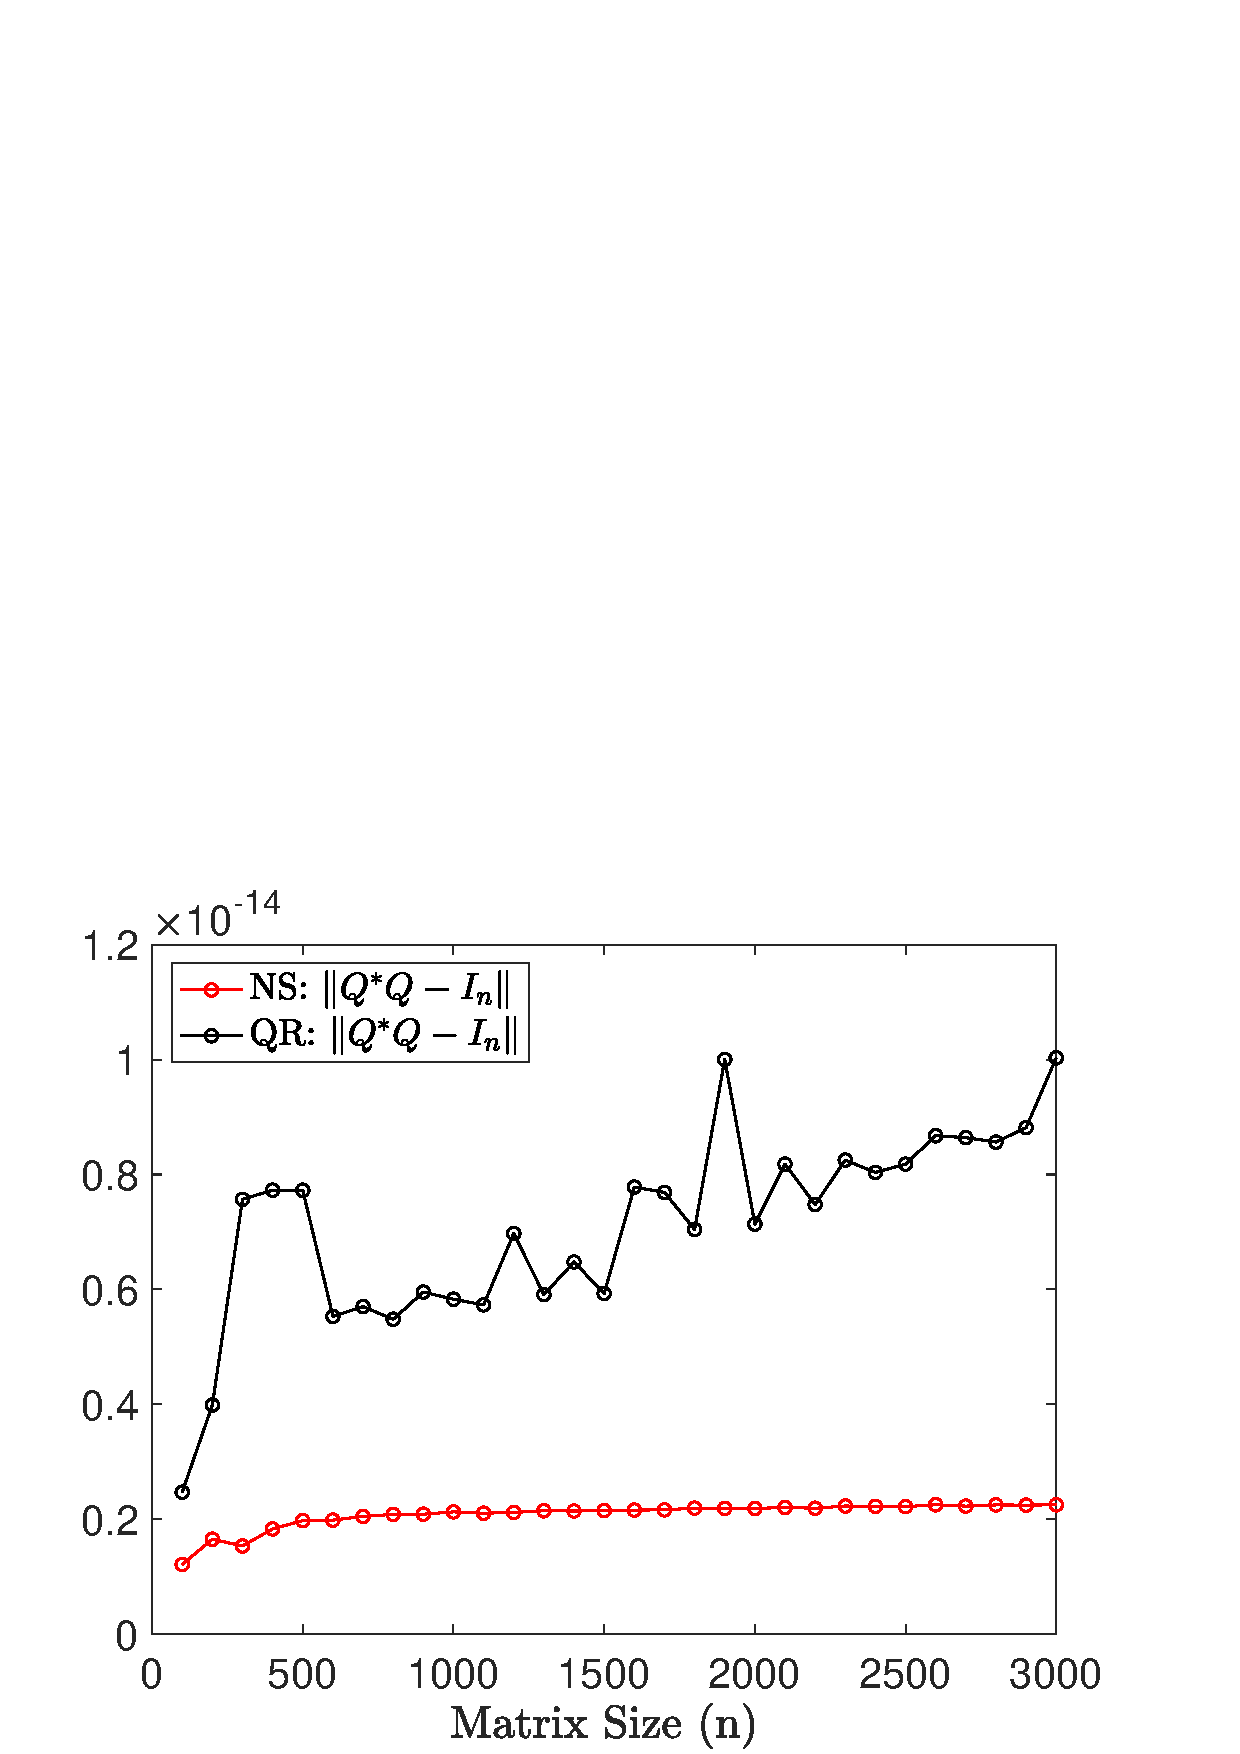
\includegraphics[width=0.5\textwidth]{figs/acccompare.pdf}
\caption[Behavior of the quantity $\norm{Q_d\ctp Q_d - I_n}$ with the dimension $n$ increases using both the QR factorization and the Newton--Schulz iteration.]{Behavior of $\norm{Q_d\ctp Q_d - I_n}$ changes as the dimension $n$ increases using both the QR factorization and the Newton Schulz iteration. The blue line shows the results using the Newton--Schulz iteration, the red line shows the results using the MATLAB built-in \inline{qr()} function and the black line shows the results using the my own QR factorization code \inline{myqr()} from Section~\ref{sec.qrtesting}. The code to regenerate this graph can be found in Appendix~\ref{app:fig:acccompare}.}
\label{fig:acccompare}
\end{figure}

From the figure, we can see that the Newton--Schulz iteration is generally more accurate than the QR factorization method. 

\subsection{Performance}\label{sec:qr-ns-performance}

The performance can be measured by the MATLAB built-in function \inline{tic} and \inline{toc}. Using similar code from Section~\ref{sec:Accuracy}, we are able to compare the time used by \inline{myqr} and \inline{newton_schulz} and produce Figure~\ref{fig:timecompare}.

\begin{figure}[ht]
\centering
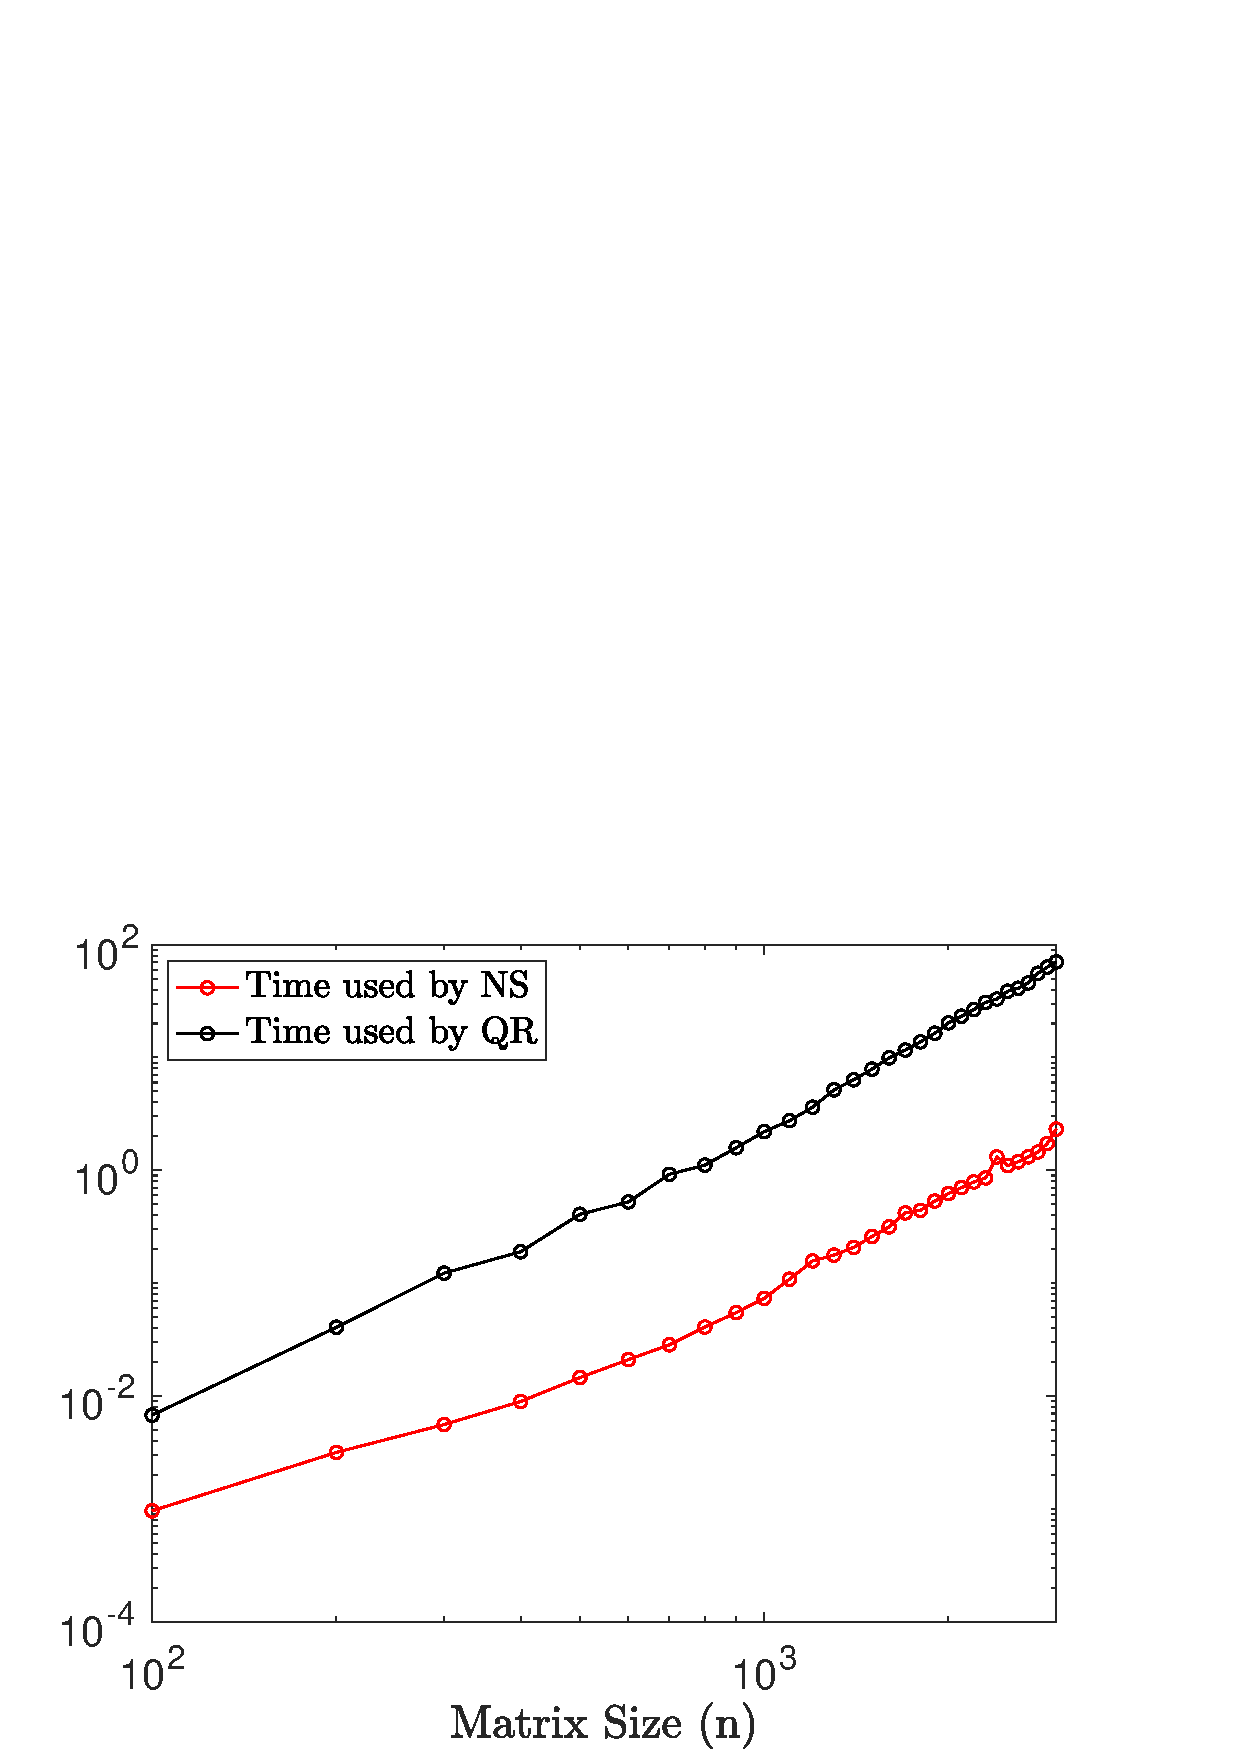
\includegraphics[width=0.5\textwidth]{figs/timecompare.pdf}
\caption[The time of applying the QR factorization and the Newton--Schulz iteration to the same almost orthogonal matrix $Q$ with respect to the dimension $(n)$.]{The time of applying the QR factorization and the Newton--Schulz iteration to the same almost orthogonal matrix $Q$. The red line shows the results using the Newton--Schulz iteration and the black line shows the results using the QR factorization. The code to regenerate this graph can be found in Appendix~\ref{app:fig:timecompare}.}
\label{fig:timecompare}
\end{figure}



From the figure, the Newton--Schulz iteration is generally faster than the QR factorization approach. 

Consequently, based on the accuracy and performance, we shall stick with the Newton--Schulz iteration approach as the method to orthogonalize the matrix $Q_\ell$.
